% !TEX root = ../../main.tex
% !TEX spellcheck = en_GB

\section{Analysis}
\label{sec:simpleanal}
\fxnote{Description of the problem and how to solve it.}
The issue of changing the frequency of a pure sine wave can be handled in a number of ways:
\begin{itemize}
	\item Changing the sampling frequency.
	\item Creating a new sine at the target frequency.
	\item Interpolating or decimating the input (only works if $f_{target}=\frac{f_{meas}}{n}\vee f_{target} =n\cdot f_{meas}$, where $n$ is an integer greater than zero.)
\end{itemize}

\paragraph{Changing the sampling frequency} is easily done in Matlab by following the recipe
\begin{enumerate}
	\item Find the input frequency.
	\item Find the ratio between the input and the target frequency.
	\item Multiply the sample frequency by the ratio between the input and target frequency.
	\item Postpad with extra samples starting at the right phase if the ratio is larger than 1. Remove samples if ratio is less than 1.
	\item Play at new sampling frequency.
\end{enumerate}
Although Matlab is able to play at different sample rates, the Blackfin has a very limited number of sample frequencies to choose from, making this approach unusable.\fxnote{Ref to design in appendix}

\paragraph{Creating a new sine at the target frequency} seems to be the most versatile possibility, as you can easily control the frequency and the phase between blocks. The drawback is that calculating the sine is an expensive operation. The steps required are
\begin{enumerate}
	\item Find the input frequency.
	\item Create new sine at target frequency.
	\item Play output sine.
\end{enumerate}

Creating a new sine at the target frequency can be made less computationally intensive by calculating sine only at some points and interpolating the rest, or using a look-up table.
It is also possible to only calculate one period of the sine at the target frequency and play that part the required number of times.
This most likely gives a phase different from 0 as the block ends, but the phase can be saved and used to calculate the sine of the next block.
This is illustrated in \cref{fig:sinblocks}, where the points from \numrange{0}{2\pi} is calculated and interpolated, but the next period from \numrange{2\pi}{4\pi} is just a copy of the period from \numrange{0}{2\pi}.
The last part creates an offset, where the phase can be determined based on the amplitude of the last two points.
This phase can then be used to create the first period of the next block.

\begin{figure}
	\centering
	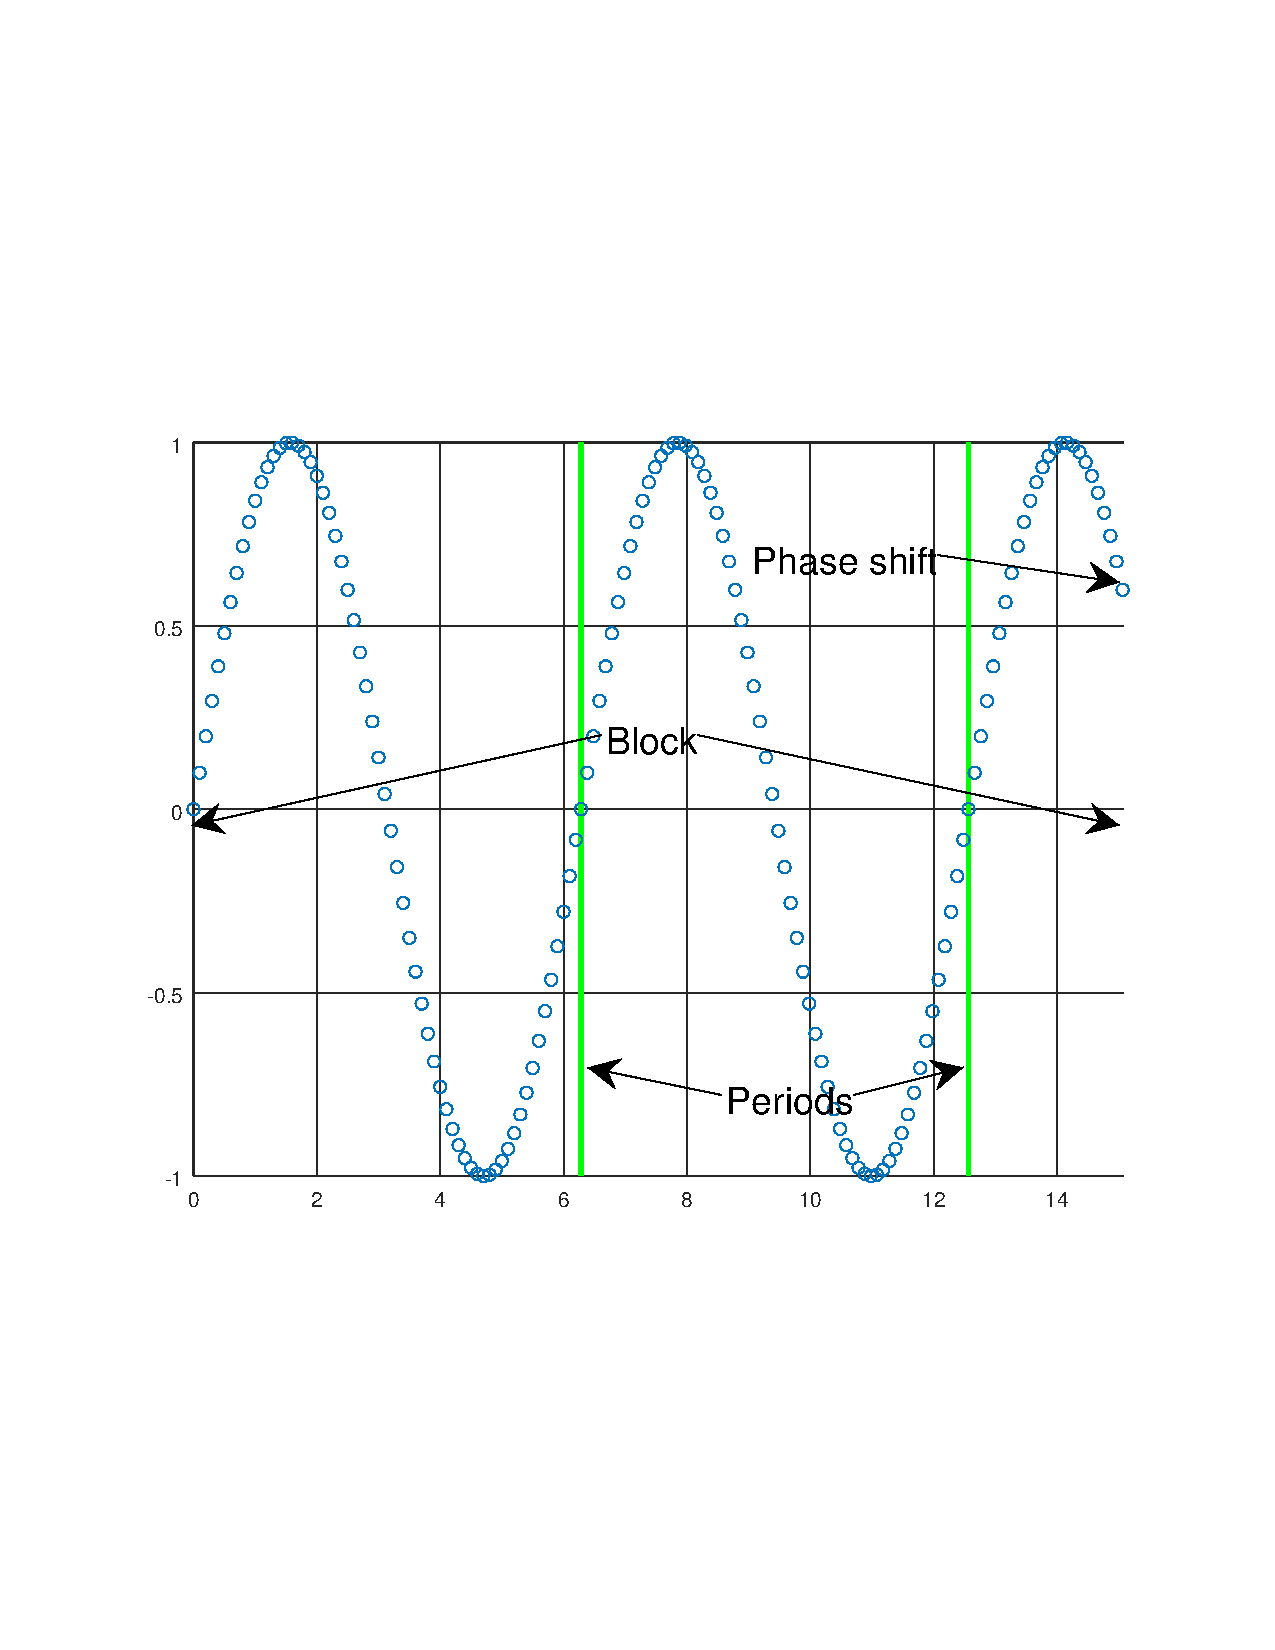
\includegraphics[width=0.7\linewidth, clip, trim={2cm 7cm 2cm 7cm}]{gfx/Analysis/SinBlocks.pdf}
	\caption{This figure shows the envisioned way of copying previously created periods, to avoid recalculation, and the ability to determine the phase for the next block to start at.}
	\label{fig:sinblocks}
\end{figure}

\paragraph{Interpolating or decimating the input} is a very simple solution, which only works if $f_{target}=\frac{f_{meas}}{n}\vee f_{target} =n\cdot f_{meas}$, where $n$ is an integer greater than zero.

\FloatBarrier